\documentclass{standalone}
    
\usepackage{tikz}
    \usetikzlibrary{arrows.meta}

\begin{document}
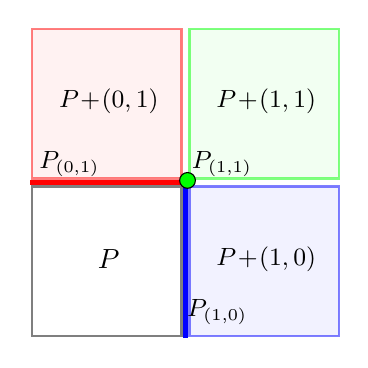
\begin{tikzpicture}
     %                                                                                                                                                                                                                                                                                                                                                                                                                                                                                                                                                                                                                                                                                                                                                                                                                                                                                                                                                                                                                                                                                                                                                                                                                                                                                                                  \draw[->,>={Latex[length=7pt]},black!50,line width=0.6mm] (0,0)--(2,2);
    % \draw[->,>={Latex[length=7pt]},black!50,line width=0.6mm] (0,0)--(2,0);
    % \draw[->,>={Latex[length=7pt]},black!50,line width=0.6mm] (0,0)--(2,-2);
    % \draw[->,>={Latex[length=7pt]},black!50,line width=0.6mm] (0,0)--(0,2);
    % \draw[->,>={Latex[length=7pt]},black!50,line width=0.6mm] (0,0)--(0,-2);
    % \draw[->,>={Latex[length=7pt]},black!50,line width=0.6mm] (0,0)--(-2,2);
    % \draw[->,>={Latex[length=7pt]},black!50,line width=0.6mm] (0,0)--(-2,0);
    % \draw[->,>={Latex[length=7pt]},black!50,line width=0.6mm] (0,0)--(-2,-2);
    \draw[opacity=0.5,line width=0.3mm,green,fill=green!10]
        % (-3,-3)++(0.025,0.025) rectangle ++(1.9,1.9)
        (1,1)++(0.025,0.025) rectangle ++(1.9,1.9);
    \draw[opacity=0.5,line width=0.3mm,blue,fill=blue!10]
        % (-3,-1)++(0.025,0.025) rectangle ++(1.9,1.9)
        (1,-1)++(0.025,0.025) rectangle ++(1.9,1.9);
    \draw[opacity=0.5,line width=0.3mm,red,fill=red!10]
        % (-1,-3)++(0.025,0.025) rectangle ++(1.9,1.9)
        (-1,1)++(0.025,0.025) rectangle ++(1.9,1.9);
    \draw[opacity=0.5,line width=0.3mm,fill=white]
        % (-3,1)++(0.025,0.025) rectangle ++(1.9,1.9)
        % (1,-3)++(0.025,0.025) rectangle ++(1.9,1.9)
        (-1,-1)++(0.025,0.025) rectangle ++(1.9,1.9);
    \draw[red,line width=.6mm] (-1,.975)--(1,.975);
    \draw[blue,line width=.6mm] (.975,1)--(.975,-1);
    \draw[fill=green] (1,1)circle(1mm);
    \node[shift={(0,0)}]{$P$}; 
    \node[shift={(2,2)}]{\small$P\!+\!(1,1)$};
    \node[shift={(2,0)}]{\small$P\!+\!(1,0)$};
    \node[shift={(0,2)}]{\small$P\!+\!(0,1)$};
    \node at (.93,.93)[above right]{\small$P_{(1,1)}$};
    \node at (-0.5,0.93)[above]{\small$P_{(0,1)}$};
    \node at (.87,-0.67)[right]{\small$P_{(1,0)}$};
\end{tikzpicture}
\end{document}